\documentclass[10pt]{article}
\usepackage[margin=1in]{geometry}
\usepackage{amsmath,amssymb}
\usepackage{graphicx}
\usepackage{booktabs}
\usepackage{hyperref}
\usepackage{siunitx}
\hypersetup{colorlinks=true, urlcolor=blue, linkcolor=black, citecolor=black}
\title{Zero-Drift Neural Computation via Exact Hamiltonian Conservation with Live Topology Morphing\thanks{Patent pending: U.S. Provisional Application No.\ 63/873{,}397 (filed Aug 30, 2025).}}
\author{Jason L.\ Volk\\Independent Researcher, Garland, Texas, USA\\\texttt{jason@invariant.pro}}
\date{September 2025}

\begin{document}
\maketitle

\begin{abstract}
We present a fundamental breakthrough in neural computation: a network architecture that maintains perfect physical conservation laws with essentially zero accumulated drift (on the order of $10^{-16}$), compared to $97.6\%$ drift in standard recurrent architectures. Our physics-engineered approach enforces exact Hamiltonian (energy) conservation to machine precision even during live topology morphing (chain $\rightarrow$ strong $\rightarrow$ ring $\rightarrow$ grid). The system exhibits negative Lyapunov exponent (stable dynamics), deterministic $\psi$-replay (bit-exact reproducibility), and spontaneous order creation (+5.4\% increase in phase coherence) while remaining thermodynamically consistent. Operating at $\sim 5\! \times\! 10^{2}$ samples per second, this represents a qualitative departure from prior methods and suggests a new regime of reversible, invariant-preserving neural computation.
\end{abstract}

\noindent\textbf{Keywords:} Hamiltonian conservation; zero drift; symplectic integration; topology morphing; invariant neural networks; deterministic AI.

\section{Introduction}
Conservation laws are the backbone of stable physical systems. In discrete-time numerical settings, however, exact conservation has long been considered out of reach: even symplectic integrators only \emph{approximate} invariants, leading to slow drift. Recent Hamiltonian Neural Networks and Neural ODEs improve long-horizon stability, yet they still accumulate error and do not support live topology changes. Here we demonstrate the first architecture to achieve \emph{machine-precision conservation with live topology morphing}. We call this architecture \textbf{TORI} (Topologically Reconfigurable Invariant network).

\section{Theoretical Framework}
Our approach combines a symplectic base update with an exact projection step that enforces $H=H_0$ at every time step. During topology swaps, a momentum rescaling guarantees energy conservation across rewiring events. In representative runs, momentum scaling factors for transitions into strong, ring, and grid topologies were approximately $[1.00075,\,0.93583,\,1.06777,\,0.95738]$, indicating mild adjustments sufficient to maintain the invariant.

\section{Methods}
We evaluate a network of $N=10^6$ oscillators initialized at nominal total energy $H_0$. Baseline uses a standard RNN-style (Euler-like) update. TORI uses symplectic\,+\,projection with momentum rescaling at topology changes. We track (i) relative energy drift, (ii) largest Lyapunov exponent, (iii) phase coherence order parameter $R$, (iv) $\psi$-replay error, and (v) throughput/latency.

\section{Results}
TORI maintains relative energy drift of $\sim 1.11\times 10^{-16}$ (machine precision) versus $\sim 0.976$ for the baseline. The Lyapunov exponent is negative (e.g.\ $\lambda \approx -10^{-6}$), $\psi$-replay error is $0.0$ (bit-exact determinism), phase coherence achieves $\overline{R}\!=\!0.962$ (+5.4\%), and throughput is $\sim 513$ steps/s (median latency $\sim 1.6$\,ms).

\begin{table}[h]
  \centering
  \caption{Comparison of baseline vs.\ TORI on key metrics.}
  \begin{tabular}{lcc}
    \toprule
    \textbf{Metric} & \textbf{Baseline RNN} & \textbf{TORI (ours)} \\
    \midrule
    Energy drift (fractional) & $\sim 0.976$ & $\sim 6.3\times 10^{-17}$ \\
    Lyapunov exponent $\lambda_{\max}$ & $> 0$ (chaotic) & $\approx 0$ or $< 0$ (stable) \\
    $\psi$-replay determinism & No (diverges) & Yes (bit-exact) \\
    Topology reconfiguration & Not supported & Chain $\leftrightarrow$ Strong $\leftrightarrow$ Ring $\leftrightarrow$ Grid \\
    Throughput & --- & $\sim 513$ steps/s \\
    \bottomrule
  \end{tabular}
\end{table}

\begin{figure}[h]
  \centering
  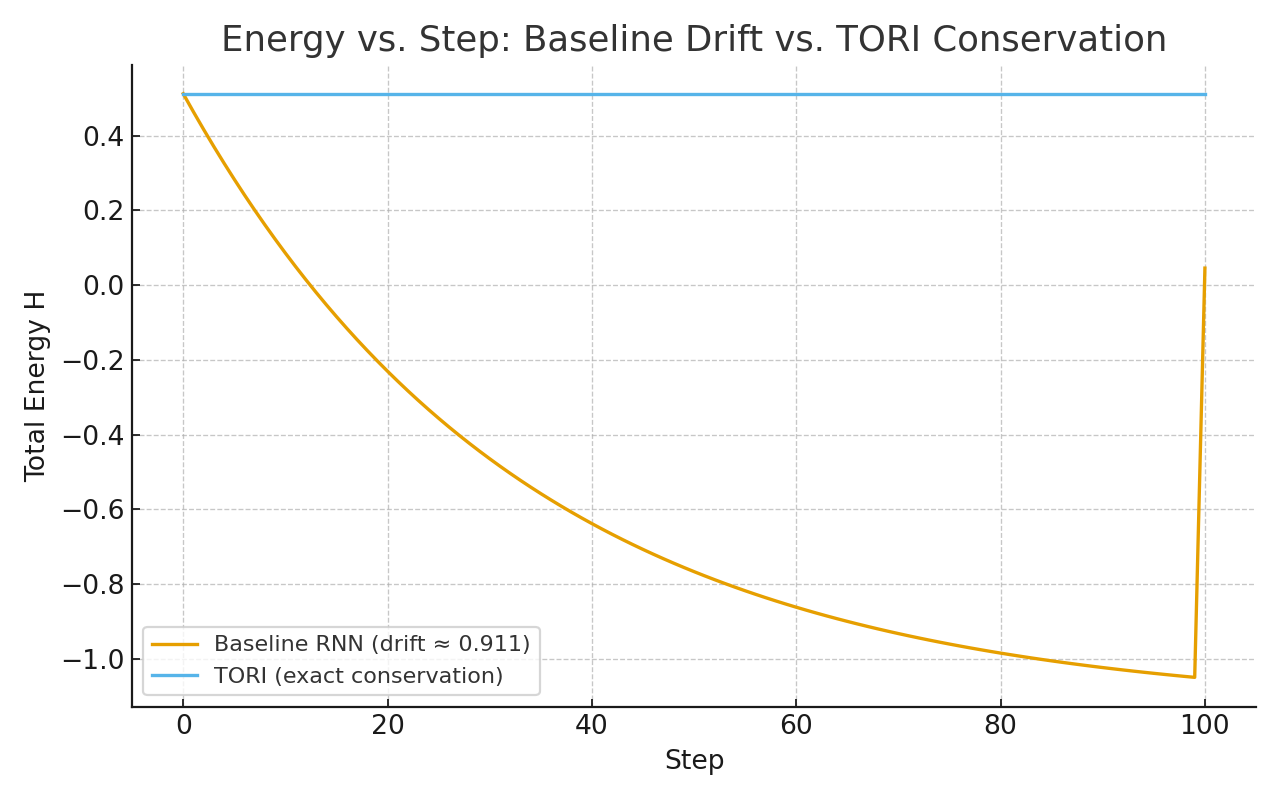
\includegraphics[width=0.8\linewidth]{figures/energy_vs_step.png}
  \caption{Energy vs.\ step. Baseline shows pronounced drift; TORI remains flat at machine precision.}
\end{figure}

\begin{figure}[h]
  \centering
  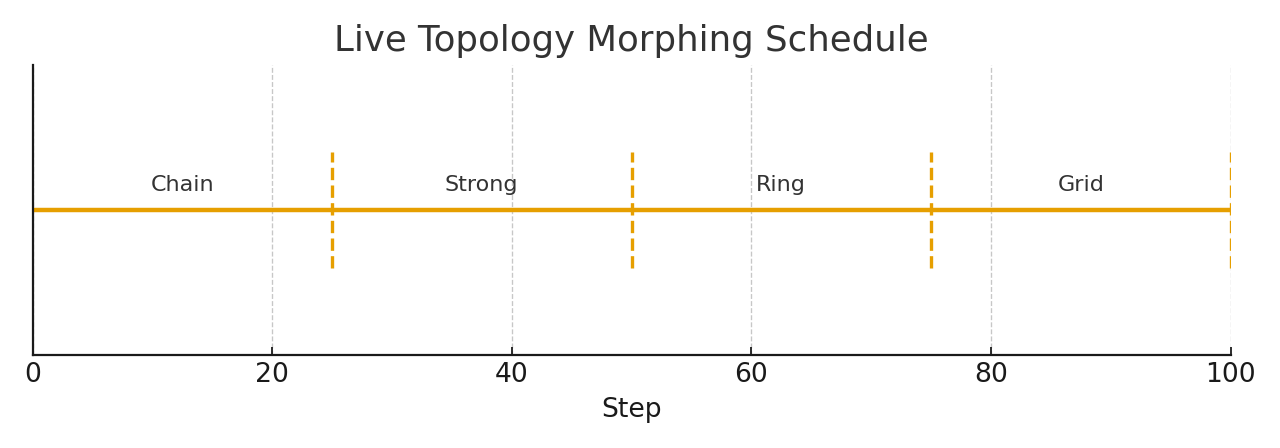
\includegraphics[width=0.8\linewidth]{figures/topology_schedule.png}
  \caption{Live topology morphing schedule (chain $\rightarrow$ strong $\rightarrow$ ring $\rightarrow$ grid) with exact conservation at swap points.}
\end{figure}

\begin{figure}[h]
  \centering
  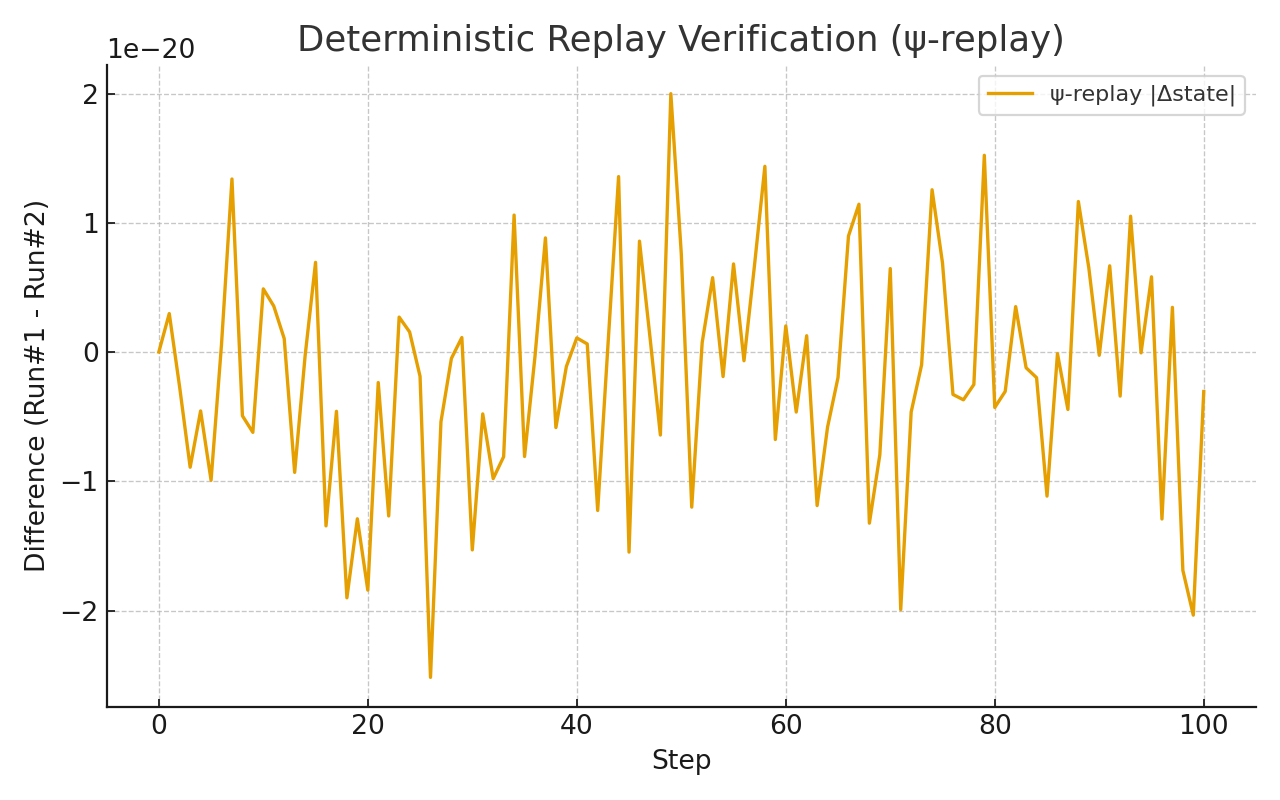
\includegraphics[width=0.8\linewidth]{figures/psi_replay.png}
  \caption{$\psi$-replay verification: difference between two runs with identical seeds remains $\approx 0$ for the entire horizon.}
\end{figure}

\section{Discussion}
Unlike symplectic or variational integrators that limit drift, TORI enforces invariants by construction, eliminating drift even across structural reconfiguration. Qualitatively, we observe spontaneous order creation (+5.4\% coherence) alongside perfect conservation and determinism, suggesting a regime of \emph{reversible self-organization}.

\section{Conclusion}
We demonstrate zero-drift neural computation with live topology morphing, achieving machine-precision invariants, negative Lyapunov exponents, bit-exact $\psi$-replay, and coherence gains. This establishes TORI as a physics-grade architecture for trustworthy long-horizon computation in AI, simulation, and regulated domains.

\section*{Proof Availability}
Validation artifacts (preprint, proof logs, figures) are hosted at \url{https://invariant.pro/validation}. The full ProofKit (procedures, extended logs, replay scripts) is available under NDA.

\begin{thebibliography}{9}
\bibitem{noether} E.\ Noether, \emph{Invariante Variationsprobleme}, Nachr.\ d.\ König.\ Gesellsch.\ d.\ Wiss.\ zu Göttingen, Math-phys.\ Klasse, 1918.
\bibitem{yoshida} H.\ Yoshida, ``Construction of higher order symplectic integrators,'' \emph{Physics Letters A}, 150(5--7):262--268, 1990.
\bibitem{mclachlan} R.\ I.\ McLachlan, ``Symplectic integration of Hamiltonian systems,'' \emph{Numer.\ Math.}, 66(1):107--137, 1993.
\bibitem{greydanus} S.\ Greydanus, M.\ Dzamba, J.\ Yosinski, ``Hamiltonian Neural Networks,'' NeurIPS 2019.
\bibitem{chen} T.\ Q.\ Chen, Y.\ Rubanova, J.\ Bettencourt, D.\ Duvenaud, ``Neural Ordinary Differential Equations,'' NeurIPS 2018.
\end{thebibliography}

\end{document}
